\textbf{5.1.} 有一能量为 5.0MeV 的质子垂直通过一均匀磁场. 设 B=1.5T, 求质子受的力.

\vfill

\textbf{5.2} 一边长为 $a$ 的正方形回路载有电流 $I$ (见习题5.2图).

(1) 求正方形中心处 B 的大小;

(2) 求正方形轴线上与中心相距为 z 的任一点处 B 的大小.

\begin{center}
    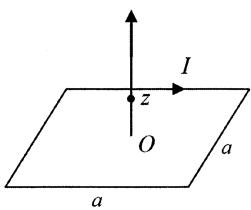
\includegraphics[width=0.3\linewidth]{figures/fig_5_4_1.jpg}
\end{center}

\vfill
\newpage

\textbf{5.3.} 一根导线折成如习题 5.3 图所示的形状, 通有电流 I, 求点 P 处 B 的大小和方向.

\begin{center}
    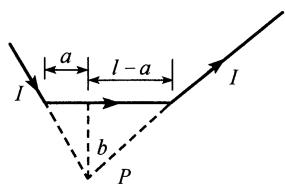
\includegraphics[width=0.3\linewidth]{figures/fig_5_4_2.jpg}
\end{center}

\vfill



\textbf{5.4.} 一导线回路是由两个径向线段连接的两个同心半圆构成(见习题5.4图)，该回路载有电流 $I$ ，求圆心处的磁场.

\begin{center}
    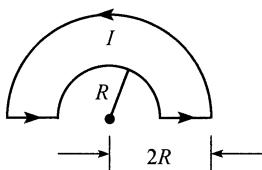
\includegraphics[width=0.3\linewidth]{figures/fig_5_4_3.jpg}
\end{center}

\vfill
\newpage

\textbf{5.5} 如习题5.5图所示，两圆线圈半径为 $R$ ，平行地共轴放置，圆心 $O_{1}, O_{2}$ 相距为 $a$ ，所载电流均为 $I$ ，且电流方向相同.

(1) 以 $O_{1}O_{2}$ 连线的中点为原点 $O$ , 求轴线上坐标为 $x$ 的任一点处的磁感应强度.

(2) 试证明: 当 a=R 时, O 点处的磁场最为均匀 (这样放置的一对线圈称作亥姆霍兹线圈, 常用它获得近似均匀的磁场.) (提示: 求磁场 B 在 x=0 处一阶和二阶导数, 证其为零).

\begin{center}
    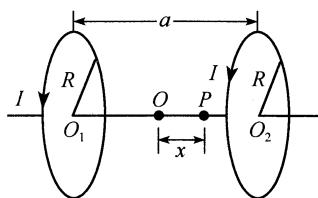
\includegraphics[width=0.3\linewidth]{figures/fig_5_4_4.jpg}
\end{center}

\vfill

\textbf{5.6.} 假定地球的磁场是由地球中心的小电流环产生的，已知地面磁极（电流环轴线与地面的交点）附近磁场为 0.8G，地球半径 $R=6\times10^{6}$ m，求小电流环的磁矩。

\vfill

\newpage

\textbf{5.7.} 螺线管线圈的直径是它的轴长的4倍，每厘米长度内的匝数 $n = 200$ ，所通电流 $I = 0.10\mathrm{A}$ ，求：

(1) 螺线管中心处磁感应强度的大小；

(2) 在管的一端中心处的磁感应强度的大小.

\vfill

\textbf{5.8.} 电流均匀地流过宽为 $2a$ 的平面导体薄板, 电流强度为 $I$ , 通过板的中线并与板面垂直的平面上有一点 $P, P$ 到板的垂直距离为 $x$ (见习题5.8图). 设板厚略去不计, 求点 $P$ 处的磁感应强度.
\begin{center}
    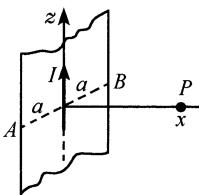
\includegraphics[width=0.25\linewidth]{figures/fig_5_10_1.jpg}
\end{center}
\vfill
\newpage

\textbf{5.9} 半径为 $R$ 的球面上均匀分布着电荷 $q$ , 该球面以角速度 $\omega$ 绕它的直径旋转, 求转轴上球内和球外任一点 (该点到球心的距离为 $z$ ) 的磁感应强度, 并求这个系统的磁矩.

\vfill



\textbf{5.10.} 如习题 5.10 图所示, 一根很长的同轴电缆, 由一导体圆柱(半径为 a) 和与之共轴的导体圆管(内、外半径分别为 b、c) 构成, 沿导体柱和导体管通以反向电流, 电流强度均为 I, 且均匀地分布在导体的横截面上, 求下述各区内的磁感应强度:

(1) 导体圆柱内 $(r<a)$ ;

(2) 两导体之间 $(a<r<b)$ ;

(3) 导体圆管内 $(b<r<c)$ ;

(4) 电缆外 $(r>c)$ .

\begin{center}
    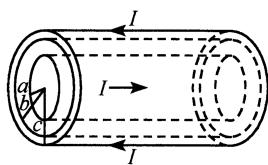
\includegraphics[width=0.25\linewidth]{figures/fig_5_10_2.jpg}
\end{center}

\vfill\newpage

\textbf{5.11.} 如习题 5.11 图所示, 一根外半径为 $R_{1}$ 的无限长圆柱形导体管, 管内空心部分的半径为 $R_{2}$ , 空心部分的轴与圆柱的轴相平行, 两轴间距离为 $a$ , 且 $a > R_{2}$ . 现有电流 $I$ 沿导体管流动, 电流均匀分布在管的横截面上, 求

(1) 圆柱轴线上的磁感应强度值；

(2) 空心部分轴线上的磁感应强度值；

(3) 设 $R_{1}=10mm, R_{2}=0.5mm, a=5.0mm, I=20A$ ，分别计算上述两处磁感应强度值。

\begin{center}
    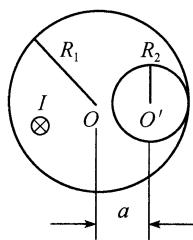
\includegraphics[width=0.15\linewidth]{figures/fig_5_12_1.jpg}
\end{center}

\vfill



\textbf{5.12.} 有两块非常大的导体板，一个在 xy 平面上，另一个在 xz 平面上，将空间划分为四个“象限”。设每块板载有均匀分布的电流，面电流密度是 i（习题 5.12 图），求各象限内的磁场。

\begin{center}
    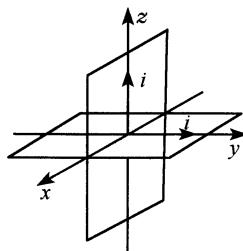
\includegraphics[width=0.2\linewidth]{figures/fig_5_12_2.jpg}
\end{center}

\vfill\newpage

\textbf{5.13.} 矩形截面的螺绕环,尺寸见习题 5.13 图,电流强度为 I,线圈总匝数为 N.

(1) 求环内磁感应强度的分布；

(2) 证明通过螺绕环截面(图中阴影区)磁通量为 $\Phi_ {B} = \left(\mu_ {0} N I h / 2 \pi\right) \ln \left(d _ {2} / d _ {1}\right)$

\begin{center}
    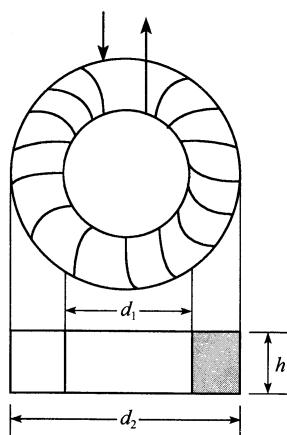
\includegraphics[width=0.2\linewidth]{figures/fig_5_15.jpg}
\end{center}

\vfill



\textbf{5.14.} 脉冲星或中子星表面的磁场有 $10^{8}\mathrm{T}$ 那样强. 考虑这样一个中子星表面上一个氢原子中的电子, 电子距质子 $0.53 \times 10^{-10}\mathrm{m}$ , 其速率是 $2.2 \times 10^{6}\mathrm{m} \cdot \mathrm{s}^{-1}$ . 试将质子作用到电子上的电力与中子星磁场作用到电子上的磁力加以比较.

\vfill\newpage

\textbf{5.15.} 一电子在 $B = 2.0 \times 10^{-3} \mathrm{T}$ 的磁场中沿半径为 $R = 2.0 \mathrm{~cm}$ 的螺旋线运动，螺距为 $h = 5.0 \mathrm{~cm}$ ，如习题5.15图所示。

(1) 求电子的速率;

(2) 确定磁场 B 的方向.

\begin{center}
    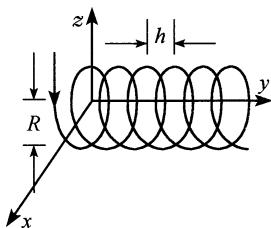
\includegraphics[width=0.3\linewidth]{figures/fig_5_16_1.jpg}
\end{center}
\vfill



\textbf{5.16.} 如习题 5.16 图所示, 一块半导体样品的体积为 $a \times b \times c$ , 沿 $x$ 方向有电流 $I$ , 在 $z$ 轴方向加有均匀磁场 $\pmb{B}$ . 已知 $a = 0.10\mathrm{cm}, b = 0.35\mathrm{cm}, c = 1.0\mathrm{cm}, I = 1.0\mathrm{mA}, B = 3000\mathrm{G}$ , 其两侧的电势差的实验结果为 $U_{AA'} = 6.5\mathrm{mV}$ .

(1) 问这半导体是正电荷导电(p型)还是负电荷导电(n型)?

(2) 求载流子浓度(即单位体积内参加导电的带电粒子数).

\begin{center}
    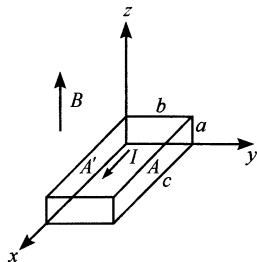
\includegraphics[width=0.3\linewidth]{figures/fig_5_16_2.jpg}
\end{center}

\vfill\newpage

\textbf{5.17.} 设在一均匀磁场 $B_{0}$ 中有一带电粒子在与 $B_{0}$ 垂直的平面内做圆周运动，速率为 $v_{0}$ ，电荷为 e，质量为 m。当磁场由 $B_{0}$ 缓慢变化到 B 时，求粒子的运动速率和回旋半径 r。

\vfill



\textbf{5.18.} 有一磁镜装置, 磁镜比为 $R_{m}=4$ , 在磁镜装置中心部位有一各向同性带电粒子